% Start preamble
\documentclass[12pt,norsk,a4paper]{book}
\usepackage[utf8]{inputenc}
\usepackage[T1]{fontenc}
\usepackage[dvips]{graphicx}
\setlength{\textwidth}{16cm}
\setlength{\oddsidemargin}{-0.5cm}
\setlength{\evensidemargin}{-0.5cm}
%\setlenght{\headsep}{0cm}
%\setlength\parindent{0pt}
%\setlength{\extrarowheight}{3pt}
%%%%%% Counting oppgaves %%%%%%
 \newcount\questnum \questnum=0
 \def\oppgave{
            \advance\questnum by 1
            \ifnum \questnum > 0
                 \hrule
                 \vskip 3pt
                 \leftline{Oppgave \the\questnum}
                 \vskip 3pt \fi}
 %%%%%%%%%%%%%%%%%%%%%%
%%%%%%%%%%%%%%%%%%%%%%


%%%%%% Counting answers %%%%%%
\newcount\answnum \answnum=0
\def\svar{
           \advance\answnum by 1
           \ifnum \answnum > 0
                \hrule
                \vskip 3pt
                \leftline{Svar \the\answnum}
                \vskip 3pt \fi}
%%%%%%%%%%%%%%%%%%%%%%


%%%%%% Counting notes %%%%%%
\newcount\explnum \explnum=0
\def\notes{
           \advance\explnum by 1
           \ifnum \explnum > 0
                \hrule
                \vskip 3pt
                \leftline{Notes \the\explnum}
                \vskip 3pt \fi}
%%%%%%%%%%%%%%%%%%%%%%

% End preamble

\begin{document}
test
%% Copyright 2010, Tony R. Kuphaldt, released under the Creative Commons Attribution License (v 1.0)
% This means you may do almost anything with this work of mine, so long as you give me proper credit

To endebrytere skal tilkobles h.h.v. \texttt{DI2} og \texttt{DI5} på en Wago 750-430 DI inngangsmodul. Tegn de nødvendige koblingene. Det internekoblingsskjemaet for (\texttt{DI1}) vises som en referanse for alle inngangene.
Tegn de nødvendige koblingene som er nødvendig for tilkobling av endebryterene.  


$$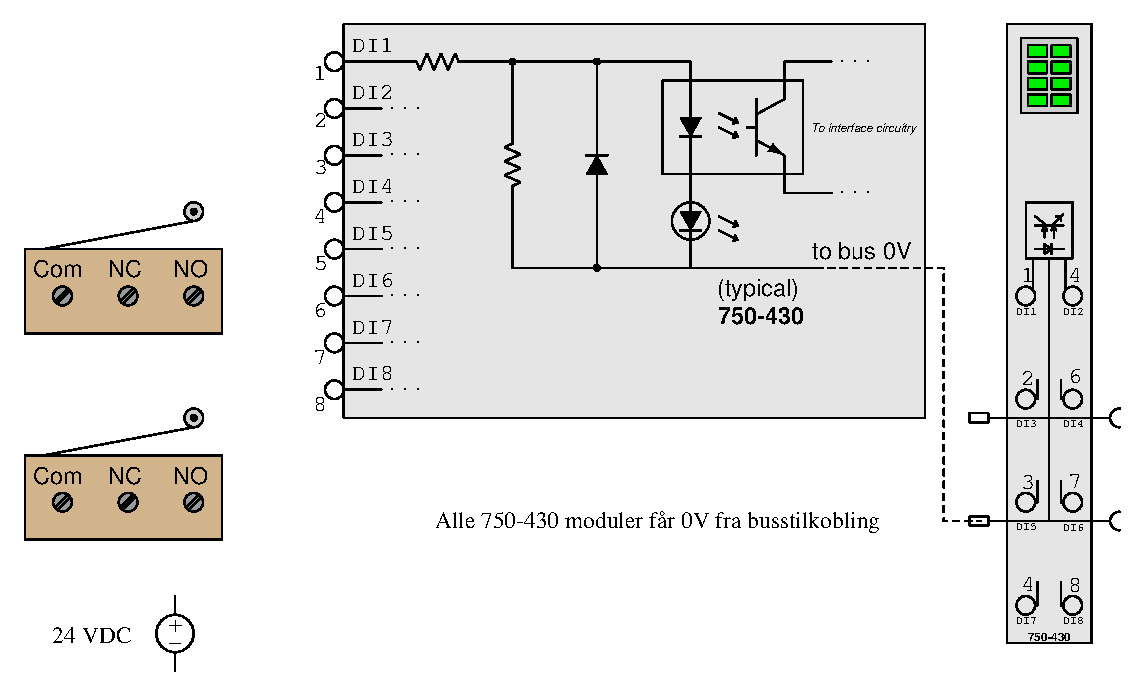
\includegraphics[width=15.5cm]{i04806x01.eps}$$

Er dette en \textit{sinking} eller en \textit{sourcing} DI modul?

\vskip 20pt \vbox{\hrule \hbox{\strut \vrule{} {\bf Suggestions for Socratic discussion} \vrule} \hrule}

\begin{itemize}
\item{} If you have identified this module as sourcing, explain how its design would differ to make it {\it sinking}.  If you have identified this module as sinking, explain how its design would differ to make it {\it sourcing}.
\item{} Explain how this module's internal circuitry could be modified to allow it to source {\it or} sink current, instead of doing just one of these functions.
\end{itemize}

\underbar{file i04806}
%(END_QUESTION)





%(BEGIN_ANSWER)

This particular input module {\it sinks} current from the limit switches (arrows drawn in the direction of conventional flow):

$$\includegraphics[width=15.5cm]{i04536x02.eps}$$



\vfil \eject



%(END_ANSWER)





%(BEGIN_NOTES)



\noindent
{\bf Prep Quiz:}

The Allen-Bradley MicroLogix 1000 PLC has the ability to either {\it source} or {\it sink} at its DC input terminals.  Determine the direction of current through each limit switch when closed:

$$\includegraphics[width=15.5cm]{i04536x03.eps}$$

Sketch or state your directions of current following {\it conventional flow} notation.




\vfil \eject

\noindent
{\bf Prep Quiz:}

This particular Allen-Bradley MicroLogix 1000 PLC has the ability to either {\it source} or {\it sink} at its relay-contact output terminals.  Determine the direction of current through each lamp when its respective output is activated:

$$\includegraphics[width=15.5cm]{i04536x04.eps}$$

Sketch or state your directions of current following {\it conventional flow} notation.










\vfil \eject

\noindent
{\bf Prep Quiz:}

Identify the stimulus condition of each switch in this PLC system, based on the color highlighting seen in the ladder-logic PLC program:

$$\includegraphics[width=15.5cm]{i04536x05.eps}$$

Level = {\it high} or {\it low}? \hskip 40pt Pressure = {\it high} or {\it low}? \hskip 40pt Flow = {\it high} or {\it low}?









\vfil \eject

\noindent
{\bf Prep Quiz:}

Identify the stimulus condition of each switch in this PLC system, based on the color highlighting seen in the ladder-logic PLC program:

$$\includegraphics[width=15.5cm]{i04536x06.eps}$$

Level = {\it high} or {\it low}? \hskip 40pt Pressure = {\it high} or {\it low}? \hskip 40pt Flow = {\it high} or {\it low}?










\vfil \eject

\noindent
{\bf Prep Quiz:}

Identify the stimulus condition of each switch in this PLC system, based on the color highlighting seen in the ladder-logic PLC program:

$$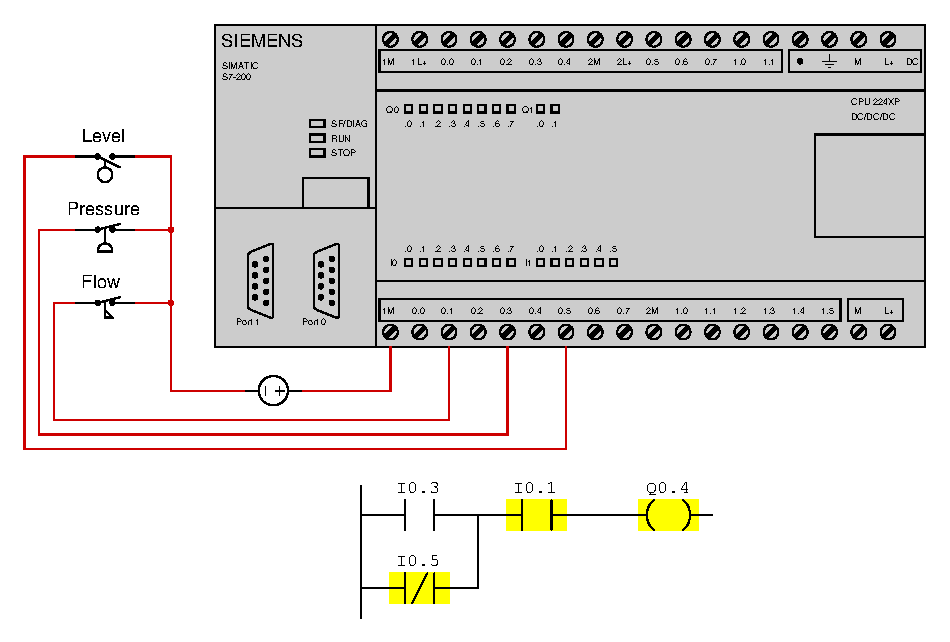
\includegraphics[width=15.5cm]{i04536x07.eps}$$

Level = {\it high} or {\it low}? \hskip 40pt Pressure = {\it high} or {\it low}? \hskip 40pt Flow = {\it high} or {\it low}?


%INDEX% PLC, I/O: discrete I/O device wiring

%(END_NOTES)




System beskrivelse

Det er 3 transportbånd, to vanlige (1 og 3) og et som kan snu (2). Transportbånd to snur rundt sin vertikale akse. Hvert transportbånd styres av en DOL startet motor. Startsignalene
for motorene er h.h.v. Motor1Fwd, Motor2Fwd og Motor2Fwd. På transportbånd 1 er det to sensorer. SensorDrop registrerer at det er ny eske på båndet og Sensor1 registrerer at det er en eske på enden av båndet. På transportbånd 2 er det to sensorer (Sensor2 og Sensor3), disse skal plassere eskene midt på og i enden av båndet. På transportbånd 3 er det to sensorer (Sensor6 og Sensor7), disse brukes til å registere eske på bånd og eske i enden av båndet. Transportbånd 2 har en motor med dreieretningsvender for snu båndet 90 grader, på denne måten kan det ta imot esker fra transportbånd 1 og levere til transportbånd 3. Sensor 4 markerer at transportbånd 2 er på linje med transportbånd 1 og Sensor 5 marker at transportbånd 2 er på linje med transportbånd 3. Det er på knapper på panelet for Start, som skal starte prosessen og og ResetSFC som restarter sekvensen.   

$$\includegraphics[width=16cm]{i04806.eps}$$
\end{document}
